%! Author = bedlamzd
%! Date = 28.02.2021

% Preamble
\documentclass[14pt]{extarticle}

%! Author = bedlamzd
%! Date = 16.02.2021

\usepackage{fontspec}
\usepackage{polyglossia}
\defaultfontfeatures{Ligatures=TeX}
\setdefaultlanguage{russian}
\setotherlanguage{english}
\setmainfont{PT Astra Serif}
\newfontfamily{\latinfont}{PT Astra Serif}
\newfontfamily{\cyrillicfont}{PT Astra Serif}
\newfontfamily{\cyrillicfonttt}{FreeMono}

\usepackage{geometry}

\usepackage{amsmath}
\usepackage{amssymb}
\usepackage{amsfonts}
\usepackage{graphicx}
\usepackage{float}
\usepackage{wrapfig}
\usepackage[caption=false]{subfig}

\geometry{right=20mm}
\geometry{left=20mm}
\geometry{top=20mm}
\geometry{bottom=20mm}

\usepackage{indentfirst}
\usepackage[outputdir=out]{minted}

\renewcommand{\theFancyVerbLine}{\ttfamily{\normalsize\oldstylenums{\arabic{FancyVerbLine}}}}

\newminted{python}{autogobble, linenos, fontsize=\small, xleftmargin=2\parindent}
\newmintinline{python}{fontsize=\small}
\newmintedfile{python}{autogobble, linenos, fontsize=\small, xleftmargin=2\parindent,
breakanywhere, breaklines}

\newminted{matlab}{autogobble, linenos, fontsize=\small, xleftmargin=2\parindent}
\newmintinline{matlab}{fontsize=\small}
\newmintedfile{matlab}{autogobble, linenos, fontsize=\small, xleftmargin=2\parindent,
breakanywhere, breaklines}

\renewcommand{\thesubsection}{\arabic{subsection}}

\graphicspath{{../img/}}



% Document
\begin{document}
    \begin{titlepage}
    \begin{center}
        \begin{small}
            \textbf{Министерство науки и высшего образования Российской Федерации}

            \vspace{1em}

            ФЕДЕРАЛЬНОЕ ГОСУДАРСТВЕННОЕ АВТОНОМНОЕ ОБРАЗОВАТЕЛЬНОЕ\\
            УЧРЕЖДЕНИЕ ВЫСШЕГО ОБРАЗОВАНИЯ

            \vspace{1em}

            \textbf{<<НАЦИОНАЛЬНЫЙ ИССЛЕДОВАТЕЛЬСКИЙ УНИВЕРСИТЕТ ИТМО>>}
        \end{small}

        \vspace{13ex}

        Практическая работа №4\\
        <<Планирование движения>>\\
        по дисциплине <<Моделирование и управление робототехническими системами>>
    \end{center}

    \vspace{14em}

    \begin{flushright}
        \noindent
        Выполнил:\\
        студент гр. R41341c\\
        Борисов М. В.

        \vspace{1em}
        Преподаватель:\\
        Каканов М. А.
    \end{flushright}

    \vfill

    \begin{center}
        \large{Санкт-Петербург}\\
        2021 г.\\
    \end{center}
\end{titlepage}


    \section*{Дано}

    \section*{Задание}
    Выполнить планирование составной траектории с четырьмя опорными точками для шестизвенного манипулятора.
    \begin{enumerate}
        \item Определить количество участков траектории
        \item Нормировать время
        \item Задать ограничения на траекторию
        \item Сформировать полиномы соответствующей степени для описания обобщённых координат, скоростей и ускорений
        \item Сформировать матричное уравнение на основе заданных полиномов и разрешить его относительно неизвестных коэффициентов
    \end{enumerate}

    \section*{Решение}
    В приложении~\ref{code:spline} приведён скрипт планирования траектории инструмента. Траектория должна проходить через четыре
    опорные точки, ограничивающие собой три участка --- сегмент ухода, сегмент собственного перемещения между рабочими зонами
    и сегмент подхода. Скорости и ускорения в опорных точках на разных участках должны совпадать из условия непрервыного
    движения.

    В качестве опорных точек зададим следующие:
    \begin{equation}
        \begin{aligned}
            \chi_1& =
            \begin{bmatrix}
                2 & 0 & 0 & 0 & 1.3090 & 3.1416
            \end{bmatrix};\\
            \chi_2& =
            \begin{bmatrix}
                2 & 0 & 2 & 0 & 0.5236 & 3.1416
            \end{bmatrix};\\
            \chi_3& =
            \begin{bmatrix}
                0 & 2 & 2 & 1.5708 & 0.5236 & 3.1416
            \end{bmatrix};\\
            \chi_4& =
            \begin{bmatrix}
                0 & 2 & 0 & 1.5708 & 1.3090 & 3.1416
            \end{bmatrix};
        \end{aligned}
    \end{equation}

    Начальные и конечные скорости и ускорения схвата манипулятора приняты нулевыми.
    Опорные значения времени примем $t = \left[1,\ 2,\ 3,\ 4 \right]$, точек на траектории 600.

    Затем для каждой опорной позиции решается ОЗК для нахождения конфигурации робота в каждом из положений.
    После вводится матрица $M$, составленная из моментов времени и коэффициентов дифференцирования.
    После чего для каждого звена, используя данную матрицу и известные ограничения, рассчитываются коэффициенты полиномов.

    Имея коэффициенты рассчитывается траектория движения манипулятора. Расчёт производится для каждого отрезка
    времени по положению, скорости и ускорению с помощью соответствующих полиномов.

    \begin{figure}[H]
        \centering
        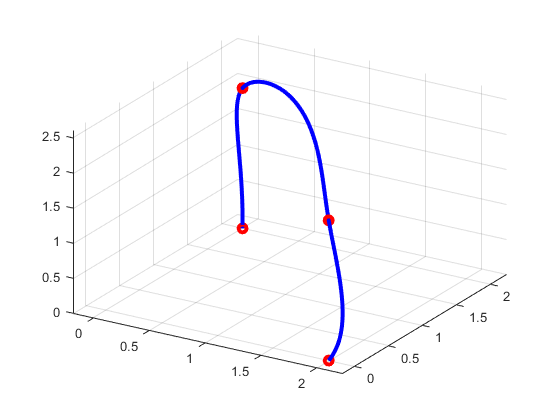
\includegraphics[width=0.75\textwidth]{traject.png}
        \caption{Траектория движения манипулятора}
        \label{pic:traject}
    \end{figure}

    По рисунку~\ref{pic:traject} видно, что траектория проходит через все обозначенные точки и плавная, что доказывает
    верность реализации.

    \section*{Вывод}
    В ходе работы реализован скрипт, строящий траекторию движения схвата манипулятора через опорные точки
    используя данные кинематики манипулятора. Полученная кривая является гладкой и не имеет точек разрыва.

    \appendix \newpage
    \renewcommand{\thesection}{\Asbuk{section}}
    \section{Функция решения прямой задачи кинематики}\label{code:spline}
    \octavefile[frame=single]{../src/spline.m}

\end{document}
